\thispagestyle{empty}
\null
\vfill
\begin{center}

   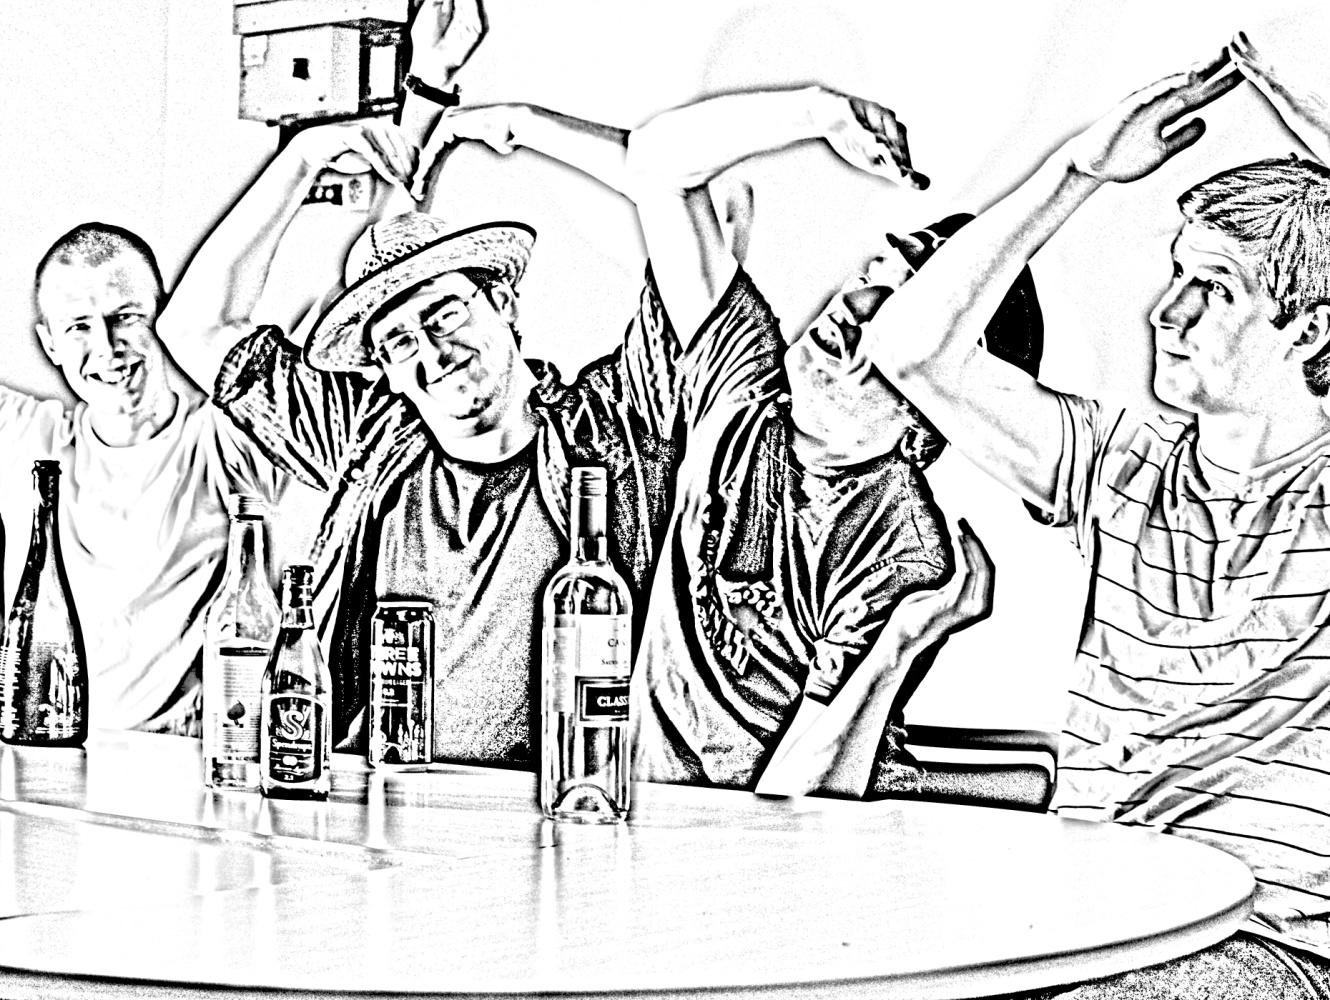
\includegraphics[width=1.0\textwidth]{res/sallskapsvisor.jpg}
   \section{Sällskapsvisor}
\end{center}
\vfill
\newpage



\subsection{Bussången}
\textit{Mel: Jag är en astronaut}\\
\index[alfa]{Bussången}
\index[anfa]{Förr när man skulle bort...}
\begin{parse lines}[\noindent]{#1\\}

Förr när man skulle bort
lång väg såväl som kort
fick man ta cykeln eller gå
nu är det inte så

Fööör...
Nu kan vi åka buss
förarn bestämmer kurs
Fönstren är många, ratten rund
här i vår buss från Lund

Nu ska vi leka bin
här i vår busskabin
Buzz, buzz, buzz, buzz, buzz, buzz, buzz, buzz
buzz, buzz, buzz, åka buss!

\end{parse lines}
\vfill
\noindent\textit{Sjungs på varje bussresa.}


\newpage
\subsection{Skolan svämmar över alla breddar}
\textit{Mel: Längtan till landet}\\
\index[alfa]{Skolan svämmar över alla breddar}
\index[anfa]{Skolan svämmar över alla breddar"!}
\begin{parse lines}[\noindent]{#1\\}

Skolan svämmar över alla breddar!
Nu har nollan åter kommit hit.
Nollan vilsen, osäker och rädd är,
ty en nolla vet ju ej ett dugg.

Irra från sektionen till KF-sigma,
famnen full av böcker; vart skall vi nu?
Festa hela natten, sen ska man pigg va;
Föreläsning börjar klockan sju!

Föreläsarn mumlar längst fram i salen,
integraler virvlar; matte är kul!
Varva fest med studier, sen kommer kvalen!
Åtta tentor, sen så är det jul!
\end{parse lines}


\subsection{Skandal}
\textit{Mel: Amazing grace}\\
\index[alfa]{Skandal}
\index[anfa]{Skandal, skandal, skandal, skandal...}
\begin{parse lines}[\noindent]{#1\\}

Skandal, skandal, skandal, skandal.
Skandal, skandal, skandal.
Skandal, skandal, skandal, skandal.
Skandal, skandal, skandal.
\end{parse lines}


\subsection{Grå häst}
\textit{Mel: Go west}\\
\index[alfa]{Grå häst}
\index[anfa]{Grå häst...}
\begin{parse lines}[\noindent]{#1\\}

Grå häst
Jag har skaffat en
Grå häst
Den är född av en
Grå häst
Den har fyra ben
Grå häst, nu så har den blivit en

Grå väst
Jag har gjort mig en
Grå väst
Den är mjuk och len
Grå väst
Den har fyra ben
Grå väst, efter tvätten blev den en

Grå rest
Den ser ut som en
Grå rest
Ganska homogen
Grå rest
Nu jag hör siren
Grå rest, myndigheten tog mig sen



Arrest
Jag är helt allen
Arrest
Nu är jag blott en
Grå rest
För de hitta en
Grå väst, Ja, jag hade stulit en

Grå häst...
\end{parse lines}

\subsection{Studiemedelsrondo}
\textit{Mel: Lossa sand}\\
\index[alfa]{Studiemedelsrondo}
\index[anfa]{Vi dricker punsch till lunch...}
\begin{parse lines}[\noindent]{#1\\}

Vi dricker punsch till lunch
när vi har fått avin.
Vi lunchar hela dagen
tills kassan gått i sin.
\end{parse lines}

\vfill
\subsection{Teknologvisa}
\textit{Mel: I'm a lumberjack}\\
\index[alfa]{Teknologvisa}
\index[anfa]{Jag är teknolog och helt OK...}

\noindent\textbf{Jag är teknolog och helt OK\\
Jag jobbar hårt och jag roar mig}\\\\
\noindent Han är teknolog och helt OK\\
Han jobbar hårt och han roar sig\\\\
\noindent\textbf{Teknik är ball\\
Jag kan Pascal\\
Till Lophtet vill jag gå\\
Där träffas alla vänner\\
som är från LTH}\\\\
\noindent Teknik är ball\\
Han kan Pascal\\
Till Lophtet vill han gå\\
Där träffas alla vänner\\
som är från LTH\\\\
\noindent För han är teknolog och helt OK\\
Han jobbar hårt och han roar sig\\\\
\noindent\textbf{Min mattebok \\
den gör mig klok\\
Jag läser kärnfysik\\
Jag går på föreläsning\\
och älskar juridik}\\\\
\noindent Hans mattebok\\
den gör han klok\\
Han läser kärnfysik\\
Han går på föreläsning\\
och älskar juridik???\\\\
\noindent Men han är teknolog och helt OK\\
Han jobbar hårt och han roar sig\\\\
\noindent\textbf{Som ekonom jag blir fantom\\
Konkurser gör mig säll\\
Till flickor blankt jag nekar\\
Jag älskar en tabell}\\\\
\noindent Som ekonom han blir fantom???\\
konkurser...\\
Nää, BUU!!\\\\
\noindent Men han är teknolog och helt OK\\
Han jobbar hårt och han roar sig\\

\noindent\textit{Fetstilt sjunges av försångare.}


\newpage
\subsection{Vi klarar oss nog ändå}
\textit{Mel: Vi klarar oss nog ändå}\\
\index[alfa]{Vi klarar oss nog ändå}
\index[anfa]{Jag vill sjunga en visa i klaraste dur...}
\begin{parse lines}[\noindent]{#1\\}

Jag vill sjunga en visa i klaraste dur,
ty den handlar om Skåne å slätter å djur.
Kan hända den retar en del,
men i så fall e det deras eget fel.
Det har talats så mycket om dynga och lort,
men betänk vilken oerhörd nytta den gjort.
Så låt dom bara gå på,
vi klarar oss nog ändå.
Ja, låt dom bara gå på,
vi klarar oss nog ändå.

Kanske språket vi talar ej klingar så väl,
men de e å förbliver en del av vår själ.
Kan hända det retar en del,
men i så fall e det deras eget fel.
Uti självaste riksdan på skånska di slåss,
för de flesta utav dom har kommit från oss.
Så låt dom ...

Hela landet får njuta av vår akvavid,
sockerbedan har lärt dom att dricka på bid.
Kan hända det retar en del,
men i så fall e det deras eget fel.
Våran sandstrand den e både bländvit å fin,
åsså har vi ju vår lilla vida kanin.
Så låt dom ..
\end{parse lines}

\vspace{-0.8cm}
\subsection{Regattasången}
\textit{Mel: Rövarna från Kamomilla stad}\\
\index[alfa]{Regattasången}
\index[anfa]{Regattaslag på LTH...}
\begin{parse lines}[\noindent]{#1\\}

Regattaslag på LTH
På sjön Sjøn ska vi härja
Förstöra allt vi kommer åt
Å dörren ska vi bärga

Båtarna körs ned på ramp
Sektionerna gör upp i kamp

Elektro Kemi Eko ING och Fysik
Data V A Maskin också I-sektion
\end{parse lines}

\vfill
\subsection{Morbid busslåt}
\textit{Mel: Båtlåt}\\
\index[alfa]{Morbid busslåt}
\index[anfa]{Det var en buss som sa till en annan...}
\begin{parse lines}[\noindent]{#1\\}

Det var en buss som sa till en annan:
- Vad du var stilig, din lack är alldeles för grann.
Vi prejas lite grann, och repar ner varann.
Som bara bussar kan.
Badda bam bam bam bam
Badda bam bam bam

Andra bussen sa: - Klart att jag vill va
med och krocka. Krossa din stiliga för.
Vi varann förstör. Busschauffören dör.
Av vägen sen vi kör.
Badda bam bam bam bam
Badda bam bam bam

Sedan kan vi slå, en och kanske två
våldsamma volter. Landa nånstans vid en bäck.
Rulla lite däck. Bensintanken är läck.
Och elden är ej släckt.
Badda bam bam bam bam
Badda bam bam BOOM!
\end{parse lines}

\newpage
\thispagestyle{empty}
\null
\vfill
\begin{center}

   
\includegraphics[width=0.8\textwidth]{res/gamlavisor.png}
   \section{Gamla visor}

\end{center}
\vfill
\newpage
\textit{Gamla visor är sånger som varit omtyckta och sjungits på sektionen, men som av olika anledningar arkiverats. Sektionen står inte bakom innehållet i visorna och de sjunges på egen risk.}

\subsection{Supa tills vi stupar}
\textit{Mel: The wild rover}\\
\index[alfa]{Supa tills vi stupar}
\index[anfa]{Vi öla på Malmö, till sång och till skrik...}
\begin{parse lines}[\noindent]{#1\\}

Vi öla på Malmö, till sång och till skrik
Då kom det en grabb, han gick juridik
Han kom fram till vårt bord, kalla oss fulla svin
men det skiter vi i för vi går på Maskin

Vi blir kvar och röjer
Kommer aldrig gå hem
Vi ska supa tills vi stupar
För vi går på M.

Vi öla i parken, då kom den en man
Han hade fått sparken, var sliten som fan
Han sa ``Läs inte data. Ni slösar bort ti'n''
men det skiter vi i för vi går på Maskin

Vi blir kvar…

Vi öla på Sparta, som så ofta har hänt
Då kom det en östtysk utbytesstudent
Han sa ``Tjänare grabbar, vill ni ha lite morfin?''
Nej det skiter vi i, TROTS att vi går på Maskin

Vi blir kvar…

Vi vakna på sjukan, hur fan kom vi dit?
Men där kom nån på här finns ju läkarsprit
Men doktorn sa ``Stopp! Det där är till medicin!''
Men det skiter vi i för vi går på Maskin

Vi blir kvar…
\end{parse lines}


\vfill
\subsection{Dunderdrickan}
\textit{Mel: Itsy bitsy}\\
\index[alfa]{Dunderdrickan}
\index[anfa]{Det var en kväll då jag gick ner till krogen...}
\begin{parse lines}[\noindent]{#1\\}

Det var en kväll då jag gick ner till krogen
för att äta å ta mig ett glas.
Första flaskan kom in och jag drog den,
sedan gick hela kvällen i kras.

``Ett, två, tre, vilken dricka var då det?''

Jo, det var en stark och mäktig dunderdricka,
tappa glaset, börja slicka.
En liten bordssup längs smalbenet rann.
En annan mäktig dunderdricka
fort slank ner, jag börja hicka.
En liten bordssup, mitt minne försvann!

Pam pam pam...

Jag är för full för att ta mig ur stolen.
Jag är för full för att känna min arm.
Jag är så full att jag trilla i poolen.
Jag vakna upp i en storbystad barm.

``Ett, två, tre, men hur kunde detta ske?''

Jo, utav en stark och mäktig dunderdricka
till akuten mig de skicka.
Min lilla bordssup gav leverbesvär.
Men doktorn på mig konstigt titta,
hitta bara sockerdricka,
och sa förbannat ``Vad fan gör du här?''
\end{parse lines}

\subsection{Efter alkohol}
\textit{Mel: The money song}\\
\textit{Bordsvisa D-sektionen 2011}\\
\index[alfa]{Efter alkohol}
\index[anfa]{Man har klagat på mitt bordsskick efter supen...}
\begin{parse lines}[\noindent]{#1\\}

Man har klagat på mitt bordsskick efter supen,
Man har anklagat mig för att sjunga falskt.
Det sägs att jag blir fumlig-
efter att min syn blir grumlig.
Men jag tar inte åt mig därför att:

Efter alkohol blir alla runt mig snygga.
Efter alkohol villa va min vän.
Ni säger:- ta det varligt
Medan jag ser inget farligt
Jag tror nog jag ska ta mig ännu en.

Efter alkohol så kan jag plötsligt flyga
Efter alkohol så vågar jag ta sats
Plötsligt blir jag modig, stark och obegripligt rolig
och allt blir möjligt genom alkohol-hol-hol

Jag må va full som fan, men du är likadan
genom öl o vin o cider
får jag alltid ragg!
\end{parse lines}

\vspace{-0.8cm}
\subsection{Här på en skola i Lund}
\textit{Mel: Under en filt i Madrid}\\
\index[alfa]{Här på en skola i Lund}
\index[anfa]{Här på en skola i Lund...}
\begin{parse lines}[\noindent]{#1\\}

Här på en skola i Lund
skulle jag studera en stund
skulle plugga och vara så sund
här på skola i Lund

För tänk innan jag kom hit
drack jag ej en droppe sprit
men här super jag som en hund
här på en skola i Lund

Min studiesituation
har upplevt en evolution
dålig är min prestation
men drycken ger motivation

I ett hav av brännvin och öl
guppar jag runt på fel köl
mina ben gör ej som jag vill
men ge mig en rackare till

För fan här finns bara drägg
kom kyss en kille med skägg
här finns inga tjejer att få
men kom ska jag få den att stå

Kanske tycker du att denna sång
bör inkapslas i en kodong
med den sagga du lade däri
men det skiter jag i

Jag skiter i studierna nu
och knullar med lärarens fru
Om varenda tenta jag kör
kan jag supa här tills jag dör

För fan där gnäggar en get
jag faller till taket som smet
det blir till att däcka en stund
här på skola i Lund
\end{parse lines}
\vfill
\subsection{Jag vill gå på Data-InfoCom}
\textit{Mel: Blommig falukorv}\\
\index[alfa]{Jag vill gå på Data-InfoCom}
\index[anfa]{Jag vill gå på Data-Infocom...}
\begin{parse lines}[\noindent]{#1\\}

Jag vill gå på Data-Infocom
Mamma
Bästa här på LTH
och alla era brudar
de dyrkar oss som gudar
Ja vi står över alla er

E - Löder för mycket
F - Pallar ej trycket
M:arna ser ut som apor

Jag vill gå på Data-Infocom
Pappa
Nått annat vill jag inte gå

Jag hatar kemister, de är som Chalmerister
A har knappt nån nollning alls

W - Dom går åt skogen
I - Snobbar på krogen
V:arna de dricker vatten

Jag vill gå på Data-Infocom
DIN MAMMA!!!
\end{parse lines}


\newpage
